\chapter{Proposed System}
\begin{justify}
    
\section{System Architecture}
The proposed system, Influencify, is a web-based platform designed to connect verified Indian influencers with brands, providing a secure, centralized environment for collaborations. It addresses key challenges in the current influencer marketing ecosystem, including transparency, secure payments, task tracking, and seamless communication. The system is highly scalable, modular, and user-friendly, enabling efficient management of influencer collaborations for both small and large-scale campaigns. The architecture is designed to support high performance, real-time interactions, and secure transactions, ensuring a smooth user experience.
The architecture of Influencify is composed of the following core components:
\begin{itemize}
    \item \textbf{Profile and Pricing Management:} Allows influencers to set pricing for different types of promotions (e.g., story posts, image uploads, video content) and manage their portfolios.
    
    \item \textbf{Search and Discovery Engine:} Enables brands to search for influencers based on filters like platform, follower count, engagement rate, and pricing, facilitating more targeted campaign planning.
    
    \item \textbf{Real-time Communication:} Powered by Firebase for instant chat functionality, ensuring timely responses and reducing communication gaps between influencers and clients.
    
    \item \textbf{Payment Processing Module:} Integrated with Razorpay or Stripe for secure, milestone-based escrow payments, ensuring fair transactions and protecting both parties.
    
    \item \textbf{Task Management and Tracking:} Provides tools for brands to send collaboration requests, track task progress, and confirm task completion before releasing payments.
    
    \item \textbf{Admin Panel:} Allows platform administrators to verify users, manage disputes, monitor transactions, and ensure platform security.
    
    \item \textbf{Analytics and Reporting:} Collects and analyzes data on influencer performance, campaign outcomes, and payment history to provide valuable insights to users.
\end{itemize}
\begin{figure}[H]
    \centering
    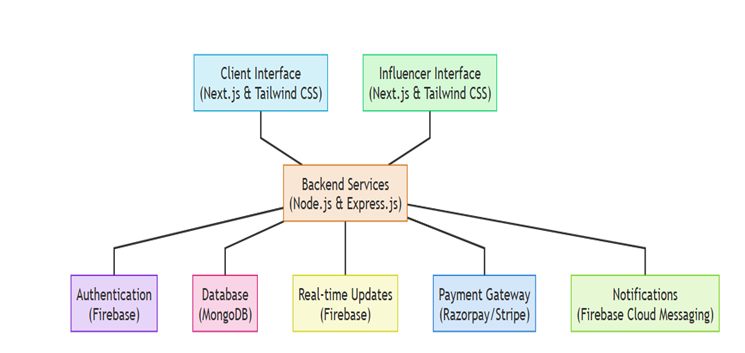
\includegraphics[height=0.3\textheight]{Chapters/Screenshot 2025-05-18 194104.png}
    \caption{System Architecture }
    \label{fig:system-workflow}
\end{figure}
\section{Features}
\subsection{Influencer Side Features}
\begin{enumerate}
    \item \textbf{Profile Creation & Management:} Influencers can create a comprehensive profile including personal information, social media links, niche, follower demographics, and engagement rates. They can update their profiles anytime to keep information current.
    \item \textbf{Pricing Setup:} Influencers set transparent prices for different promotion types such as story uploads, image posts, and video posts. Pricing can vary by platform (Instagram, YouTube, Facebook, etc.) and content type, allowing flexibility.
    \item	\textbf{Platform Selection:} Influencers specify on which platforms they want to offer promotions, helping clients filter based on campaign requirements.
    \item 	\textbf{Chat Requests:} Influencers receive and manage incoming chat requests from potential clients. The chat system supports real-time messaging to discuss campaign details efficiently.
    \item \textbf{Request Management:} Influencers can accept or reject promotion requests based on availability, campaign relevance, or other criteria.
    \item \textbf{Earnings & Payment History:} A detailed dashboard displays earnings, pending payments, transaction history, and milestone payments, providing full transparency.
    \item 	\textbf{Influencer-to-Influencer Collaboration:} Enables co-creation opportunities where influencers can collaborate on campaigns, share audiences, and increase organic reach.
\end{enumerate}
\subsection{Client Side Features}
\begin{enumerate}
    \item \textbf{Influencer Search & Filtering:} Clients can search influencers using filters like niche, platform, follower count, engagement rate, and pricing to find the best fit for their campaign.
    \item 	\textbf{Profile & Package Viewing:} Clients can view detailed influencer profiles, including previous work, reviews, and promotional packages.
    \item 	\textbf{Direct Chat:} Secure and real-time messaging with influencers to discuss campaign specifics, timelines, and deliverables.
    \item 	\textbf{Promotion Requests:} Clients can send promotion requests to influencers, outlining the campaign details and expectations.
    \item 	\textbf{Secure Payment System:} Payments are made securely through milestone-based escrow. Funds are held until campaign deliverables are approved.
    \item 	\textbf{Task Approval:} Clients review completed promotion posts and approve or dispute the work before payment is released.
\end{enumerate}
\subsection{Admin Side Features}
\begin{enumerate}
    \item 	\textbf{User Verification:} Admins verify authenticity of both influencers and clients through document checks, social media audits, and activity monitoring to maintain platform trust.
    \item 	\textbf{Monitoring & Moderation:} Admins monitor chats and promotion requests for policy compliance and fraud prevention.
    \item 	\textbf{Payment Tracking:} Oversees all payment transactions including escrow management, payment releases, refunds, and disputes.
    \item 	\textbf{Dispute Resolution:} Admins intervene in case of payment or content disputes, providing fair resolutions to maintain platform integrity.
    \item 	\textbf{Notification Management:} Admins can send targeted notifications and alerts to users about campaign updates, policy changes, or platform news.
\end{enumerate}
\section{Workflow}
\begin{enumerate}
\item \textbf{	Influencer Registration & Profile Creation: }Influencers sign up and complete their profile, including pricing and platform preferences.
\item 	\textbf{Client Browsing & Searching:} Clients search for influencers based on campaign needs using filters.
\item 	\textbf{Sending Promotion Requests:} Clients send detailed promotion requests to selected influencers.
\item 	\textbf{Influencer Response:} Influencers review requests and either accept or reject them.
\item 	\textbf{Payment Process Initiation:} Upon acceptance, clients make payment to the platform’s escrow system.
\item 	\textbf{Content Creation & Posting:} Influencers complete the promotional task by posting the agreed content on their platform(s).
\item 	\textbf{Client Approval:} Clients verify the content and approve or request modifications.
\item 	\textbf{Payment Release:} After client approval, funds are released from escrow to the influencer within 7 days.
\item \textbf{	Post-Campaign Review & Rating:} Both parties can rate and review each other to build platform credibility.
\end{enumerate}
\begin{figure}[H]
    \centering
    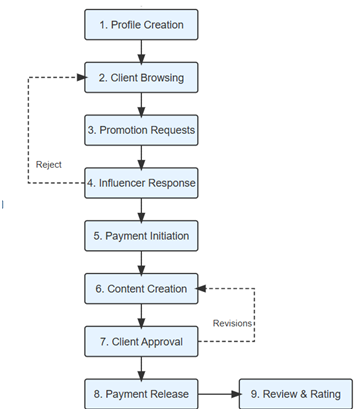
\includegraphics[height=0.4\textheight]{Chapters/Screenshot 2025-05-18 193856.png}
    \caption{Workflow of the System}
    \label{fig:system-workflow}
\end{figure}
\section{Components}
\subsection{Frontend:}
\begin{enumerate}
    \item Built with Next.js for server-side rendering and static generation, improving SEO and performance.
    \item Uses Tailwind CSS and CSS Modules for modular, responsive, and maintainable styling.
    \item Handles user interactions, profile management, search, chat UI, and payment interfaces.
\end{enumerate}
\subsection{Backend:}
\begin{enumerate}
    \item 	Developed with Node.js and Express.js to provide RESTful API endpoints.
    \item 	Manages authentication, business logic, campaign management, payment processing, and real-time notifications.
    \item 	Integrates with external services for payments and messaging.
\end{enumerate}
\subsection{Database:}
\begin{enumerate}
    \item MongoDB stores user data, campaign details, chat logs, and transaction records in flexible JSON-like documents.
    \item Ensures fast querying, indexing, and scalability for growing user base.
\end{enumerate}
\subsection{Real-Time Communication:}
\begin{enumerate}
    \item 	Uses Firebase Realtime Database for instant chat message synchronization across devices.
    \item 	Supports offline persistence and automatic sync when connectivity is restored.
\end{enumerate}
\subsection{Authentication:}
\begin{enumerate}
    \item Employs Firebase Authentication supporting Google Sign-In and email/password login.
    \item 	Ensures secure session management and role-based access control.
\end{enumerate}
\subsection{Payment System:}
\begin{enumerate}
    \item Integrates Razorpay and Stripe to process secure milestone-based escrow payments.
    \item	Manages payment releases, refunds, multi-currency support, and transaction tracking.
\end{enumerate}
notifications for chats, campaign updates, payments, and alerts.
    \begin{figure}[H]
    \centering
    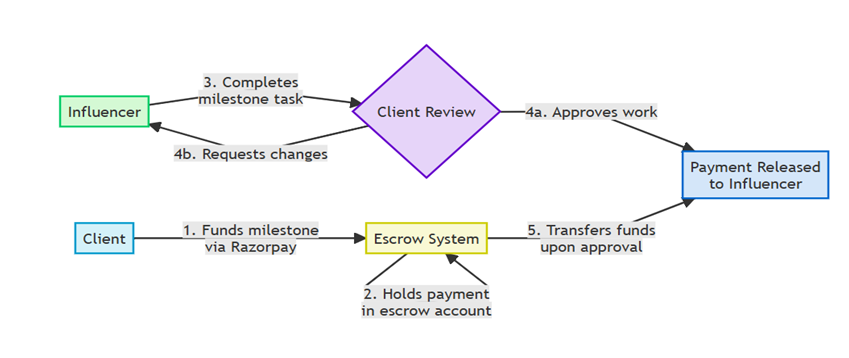
\includegraphics[height=0.3\textheight]{Chapters/Screenshot 2025-05-18 194646.png}
    \caption{Escrow Payment Flow}
    \label{fig:system-workflow}
\end{figure}
\subsection{	Notification System:}
	Uses Firebase Cloud Messaging (FCM) to send real-time push 
\section{Limitations of Existing Solutions}

\begin{itemize}
    \item \textbf{Lack of Trust and Verification:}
    Many influencer platforms do not verify the credibility of influencers or brands, which can result in fraud, fake profiles, or unreliable partnerships.
    Influencify provides a verified platform where both influencers and clients go through a rigorous verification process. Influencers can showcase their real social media metrics and profiles, ensuring that both parties can trust each other’s legitimacy.
    
    \item \textbf{Fragmented Communication:}
    Influencers and brands often communicate via informal channels like social media DMs, leading to miscommunication, delays, or misunderstandings. There’s no centralized record of conversations.
    Influencify integrates in-app chat functionality using Firebase Realtime Database, which allows clients and influencers to directly communicate within the platform. All conversations are logged, ensuring that there’s a clear, transparent record of discussions and agreements.

    \item \textbf{Unreliable Payment Systems:}
    Influencers face delayed or inconsistent payments after completing promotional tasks, and platforms often lack a secure and transparent payment process.
    Influencify uses a secure escrow payment system through integrated payment gateways like Razorpay or Stripe. The payment is held in escrow until the influencer completes the task, and only when the client confirms the work, is the payment released to the influencer. This ensures fair and timely transactions for both parties.

    \item \textbf{Limited Customization for Clients:}
    Existing platforms may not offer the right tools for clients to filter and find influencers who match their specific needs, or to customize promotion packages.
    Clients on Influencify can search and filter influencers based on multiple parameters such as category, platform, followers, price range, and more. Additionally, clients can send customized promotion requests based on specific requirements, ensuring a better match between the brand and influencer.

    \item \textbf{Absence of Task Tracking and Milestones:}
    Many platforms fail to provide a structured system for task tracking, leading to confusion about deliverables and timelines.
    Influencify introduces a milestone-based system where each task is tracked from creation to completion. Influencers and clients both know what’s expected, and payments are only processed after the client confirms the deliverables. This reduces ambiguity and ensures smoother workflows.

    \item \textbf{Inefficient Dispute Resolution:}
    In case of issues or disagreements, many platforms offer minimal dispute resolution support, leaving users to handle conflicts without clear processes.
    Influenciy includes a dispute resolution system where the admin team can intervene if any issues arise between influencers and clients. This ensures that both parties have a neutral, fair process to address conflicts and concerns.

    \item \textbf{No Collaboration Opportunities:}
    Many platforms don’t encourage collaboration between influencers, missing the potential for co-created campaigns and organic growth.
    Influencify promotes influencer-to-influencer collaborations, where influencers can connect with each other to collaborate on campaigns, exchange ideas, and co-create content. This not only benefits influencers but also fosters organic growth and cross-promotion.
\end{itemize}
\end{justify}
